Con el propósito de desarrollar la solución de Mie, se comenzará por una breve revisión de algunos conceptos fundamentales del electromagnetismo. De esta forma, se establecerán las convenciones que serán usadas a lo largo de estas notas y, además, servirá como un punto de partida para el desarrollo del problema de esparcimiento.

\section{Ecuaciones de Maxwell}

Los fenómenos electromagnéticos son descritos casi por completo a través un conjunto de cuatro ecuaciones conocidas como \textit{ecuaciones de Maxwell}. Con ellas se determina el comportamiento y la propagación de los campos electromagnéticos y cómo son influenciados por fuentes externas~\cite{Jackson}. En el caso donde los campos eléctrico $\vb{E}$ y magnético $\vb{B}$ se propagan en el vacío las ecuaciones de Maxwell se escriben como~\cite{Jackson}:
%
	\begin{tcolorbox}[title = Ecuaciones de Maxwell en el vacío]\vspace*{-0.3cm}
\begin{flalign}
	&  & \div \vb{E} &= \frac{\rho_{tot}}{\epsilon_{0}}, &  & \text{Ley de Gauss eléctrica} \label{eq:maxwell1}\\
	&  & \div \vb{B} &= 0, &  & \text{Ley de Gauss magnética} \label{eq:maxwell2}\\
	&  & \curl \vb{E} &= - \pdv{\vb{B}}{t}, &  & \text{Ley de Faraday--Lenz} \label{eq:maxwell3}\\
	&  & \curl \vb{B} &= \mu_{0} \vb{J}_{tot}+ \epsilon_{0} \mu_{0} \pdv{\vb{E}}{t}, &  & \text{Ley de Amp\`ere--Maxwell}\label{eq:maxwell4}
\end{flalign}
\end{tcolorbox}
%
\noindent en donde $\epsilon_{0}$ es la permitividad eléctrica del vacío, mientras que $\mu_{0}$ es la permeabilidad magnética del vacío; $\rho_{total}$ se refiere a la densidad volumétrica de carga total y $\vb{J}_{tot}$ a la densidad volumétrica de corriente total. Es importante destacar que las Ecs.~\eqref{eq:maxwell1}--\eqref{eq:maxwell4} están escritas en unidades del sistema internacional. Cada una representa una expresión matemática que describe observaciones experimentales. No pueden ser demostradas pero su aplicabilidad es verificable, por ello, las ecuaciones de Maxwell se utilizan en diversos problemas que involucren sistemas macroscópicos~\cite{Reitz}.

Las Ecs.~\eqref{eq:maxwell1} y.~\eqref{eq:maxwell4} cambian su forma cuando los campos electromagnéticos se propagan en medios materiales. Para ello, es necesario considerar al vector de desplazamiento, definido como~\cite{Jackson}:
\begin{equation}
\vb{D} = \epsilon_{0} \vb{E} + \vb{P},
\label{eq:vecDes}
\end{equation}
con $\vb{P}$ la polarización del material, y al campo $\vb{H}$, cuya relación con el campo magnético es~\cite{Griffiths}:
\begin{equation}
\vb{H} = \frac{\vb{B}}{\mu_{0}}-\vb{M}.
\label{eq:campoH}
\end{equation}
donde $\vb{M}$ corresponde a la magnetización del medio material. Por tanto, las ecuaciones de Maxwell en medios materiales son~\cite{Jackson}:
\begin{tcolorbox}[title = Ecuaciones de Maxwell en medios materiales]\vspace*{-0.3cm}
\begin{subequations}
	\begin{align}
		\div \vb{D}& = \rho_{ext},\label{eq:maxwell1_mat}\\
		\div \vb{B}& =0,\\
		\curl \vb{E}& = - \pdv{\vb{B}}{t},\\
		\curl \vb{H} &= \vb{J}_{ext} + \pdv{\vb{D}}{t},
		\label{eq:maxwell4_mat}
	\end{align}
\end{subequations}
\end{tcolorbox}
\noindent en donde $\rho_{ext}$ corresponde a la densidad de carga volumétrica externa y $\vb{J}_{ext}$ es la densidad de corriente volumétrica externa. 

Las ecuaciones de Maxwell en para medios materiales  [Ecs.~\eqref{eq:maxwell1_mat}--\eqref{eq:maxwell4_mat} contienen la información del material a través de dos cantidades conocidas como polarización, $\vb{P}$, y magnetización, $\vb{M}$~\cite{Griffiths}. Por ello, es preciso contar con relaciones que describan el comportamiento de los materiales bajo la influencia del campos EMs. En general, la polarización y magnetización no se pueden describir en una forma reducida y simple. Sin embargo, pueden realizarse algunas suposiciones sobre el material en cuestión. El caso más sencillo consiste en un medio material que cumple con ser \textit{homogéneo} (sus propiedades son iguales en cada punto), \textit{isotrópo} (sus propiedades ópticas en cada punto son independientes de la dirección) y tiene una respuesta ante los campos EMs de tipo \textit{lineal}. Dichas características permiten escribir \textit{relaciones constitutivas} que establecen una relación entre los cuatro campos vectoriales $\vb{E}$, $\vb{B}$, $\vb{D}$ y $\vb{H}$, La polarización y la magnetización cumplen con~\cite{Griffiths}:
%
\begin{eqnarray}
	\vb{P}=\epsilon_{0}\chi_{e}\vb{E},\qquad \vb{M}=\chi_{m}\vb{H},\label{eq:rel_constitutivas}
\end{eqnarray} 
%
respectivamente, donde se ha utilizado que $\chi_{e}$ ($\chi_{m}$) es la susceptibilidad eléctrica (magnética). De está forma, al sustituir las Ecs.~\eqref{eq:rel_constitutivas} en las expresiones para los campos $\vb{D}$ [Ec.~\eqref{eq:vecDes}] y $\vb{H}$ [Ec.~\eqref{eq:campoH}], se llega a~\cite{Griffiths}
\begin{eqnarray}
	\vb{D}=\epsilon\vb{E}, \qquad \text{y} \qquad
	\vb{H}=\frac{1}{\mu} \vb{B}, \label{eq:hache}
\end{eqnarray}
donde  $\epsilon\equiv\epsilon_{0}\left(1+\chi_{e}\right)$ y $\mu\equiv\mu_{0}\left(1+\chi_{m}\right)$ son la permitividad y permeabilidad características del medio material, respectivamente. En general, $\epsilon$ es una cantidad compleja que depende de la frecuencia de la onda incidente. A partir de ambas propiedades se expresa el índice de refracción del material en cuestión~\cite{Griffiths}
%
\begin{equation}
	n\equiv\sqrt{\frac{\epsilon\mu}{\epsilon_{0}\mu_{0}}}.
\end{equation}

\section{Condiciones a la frontera}
Las ecuaciones de Maxwell son ecuaciones diferenciales aplicadas localmente en cada punto del espacio~\cite{Jackson}. EN particular, es interesante conocer lo que sucede con las componentes de los campos $\vb{E}$, $\vb{B}$, $\vb{D}$ y $\vb{H}$ en la interfaz que separa dos medios. Para ello se inicia escribiendo a las ecuaciones de Maxwell en su forma integral~\cite{Griffiths}
\begin{subequations}
	\begin{align}
		\oint_{S}\vb{D}\cdot\dd{\vb{a}}&=Q_{tot},\label{MaxwellInt1}\\
		\oint_{S}\vb{B}\cdot\dd{\vb{a}}&=0,\label{MaxwellInt2}\\
		\oint_{P}\vb{E}\cdot\dd{\vb{l}} &=- \dv{}{t}\int_{S}\vb{B}\cdot\dd{\vb{a}},\label{MaxwellInt3}\\
		\oint_{P}\vb{H}\cdot\dd{\vb{l}}&=I_{tot}+\dv{}{t}\int_{S}\vb{D}\cdot\dd{\vb{a}}\label{eq:MaxwellInt4},
	\end{align}
\end{subequations}

Con el propósito de derivar estudiar la continuidad de los campos en una interfaz, primero, se suponen dos medios, cada uno caracterizado por sus propiedades ópticas: $\epsilon_{1},\:\mu_{1}$ para el medio 1 y $\epsilon_{2},\:\mu_{2}$ para el medio 2. La interfaz que separa ambos medios tiene densidad superficial de carga $\sigma_{tot}$ y una densidad superficial de corriente $\vb{K}_{tot}$. En particular, para analizar las componentes de $\vb{D}$ ortogonales a la interfaz, se realiza la integral en la Ec.~\eqref{MaxwellInt1}. Para ello, se elige un prisma rectangular como el que se muestra en la Fig.~\ref{fig:BoundaryConditions}(a) (conocido como \textit{Gaussian pillbox}); se supondra que su altura es $\delta$ y que sus caras paralelas a la superficie tienen un área $A$. Una parte del volumen estará por encima de la interfaz y el resto se encontrará por debajo. El vector normal a la superficie está denotado por $\vu{n}$. Puesto que la integral en la Ec.~\eqref{MaxwellInt1} es de superficie, se realiza sobre todas las caras del volumen. Sin embargo, se considera que la altura de la caja es infinitesimalmente pequeña ($\delta\to 0$). Por tanto, sólo las caras de área $A$ contribuyen, dando como resultado~\cite{Griffiths}: 
\begin{equation}
\begin{split}
\oint_{S}\vb{D}\cdot\dd{\vb{a}}=\left(D_{1}^{\perp}-D_{2}^{\perp}\right)A=Q_{enc},\label{eq:int1}
\end{split}
\end{equation}
donde $D_{1}\perp$ y $D_{2}^{\perp}$ corresponden a las componentes del vector de desplazamiento ortogonales a la interfaz en los medios 1 y 2, respectivamente. Ademas, $Q_{enc}$ es la carga encerrada por el volumen de la caja. Recordando que $Q_{enc}=\sigma_{enc}A$, se puede reescribir a la Ec.~\eqref{eq:int1} en términos de la densidad de carga superficial:
\begin{equation}
D_{1}^{\perp}-D_{2}^{\perp}=\sigma_{tot}.
\end{equation}
Por tanto, la componente perpendicular del campo $\vb{D}$ es discontinua en la frontera entre dos medios.
%\begin{equation}
%	\vb{D}_{1}\cdot \vb{A}-\vb{D}_{2}\cdot \vb{A}=\sigma_{tot}A
%\end{equation}
A través de un procedimiento similar y usando la Ec.~\eqref{MaxwellInt2}, se deduce que~\cite{Griffiths}
\begin{equation}
B_{1}^{\perp}-B_{2}^{\perp}=0,
\end{equation}
donde $B_{i}^{\perp}$ denota la componente del campo $\vb{B}$ perpendicular a la interfaz dentro del medio $i=1,\:2$. Es decir, la componente perpendicular del campo $\vb{B}$ es continua a través de la frontera.

Por otro lado, a partir de la Ec.~\eqref{MaxwellInt3} es posible describir la continuidad de las componentes del campo eléctrico paralelas a la interfaz. Con ese fin, la integral de trayectoria en la Ec.~\eqref{MaxwellInt3} se calcula utilizando un circuito rectangular como el mostrado en la Fig.~\ref{fig:BoundaryConditions}(b); su altura  es $\delta$ y el ancho $l$. Nuevamente, la mitad del circuito se encuentra inmerso en el medio 1 (sobre la interfaz) y el resto en el medio 2 (debajo de la interfaz). Se considerará el límite $\delta\to0$, por tanto, la integral queda como
\begin{equation}
\oint_{P}\vb{E}\cdot\dd{\vb{l}}=(E_{1}^{\parallel}-E_{2}^{\parallel})l=\vb{E}_{1}\cdot\vb{l}-\vb{E}_{2}\cdot\vb{l},
\end{equation}
siendo $E_{1}^{\parallel}$ y $E_{2}^{\parallel}$ las componentes del campo eléctrico paralelas a la superficie de la interfaz en los medios 1 y 2, respectivamente. Por otra parte, al considerar que la altura del circuito es infinitamente pequeña la contribución del campo magnético a la Ec.~\eqref{MaxwellInt3} es despreciable. Esto último puede entenderse al considerar que la integral de superficie del campo $\vb{B}$ da como resultado $B_{\perp}A^{*}$, con $A^{*}$ el área del circuito. Al realizar el límite $\delta\to0$, el área también tiende a cero. Por tanto, se concluye que~\cite{Griffiths}
\begin{equation}
\vb{E}^{\parallel}_{1}-\vb{E}^{\parallel}_{2}=\vb{0},
\end{equation}
es decir, los componentes del campo eléctrico paralelas a la interfaz son continuas sobre la frontera. 

De la Ec.~\eqref{eq:MaxwellInt4} se deduce una relación para las componentes del campo $\vb{H}$. Utilizando el circuito ya descrito, se realiza la integral de contorno~\cite{Griffiths}:
\begin{equation}
\oint_{S}\vb{H}\cdot\dd{\vb{l}}=(H^{\parallel}_{1}-H^{\parallel}_{2})l=\vb{H}^{\parallel}_{1}\cdot\vb{l}-\vb{H}^{\parallel}_{2}\cdot\vb{l},
\end{equation}
donde $H_{1}^{\parallel}$ y $H_{2}^{\parallel}$ son las componentes del campo eléctrico paralelas a la superficie de la interfaz en los medios 1 y 2, respectivamente. Se debe notar que la contribución del campo $\vb{D}$ a la Ec.~\eqref{eq:MaxwellInt4} es despreciable debido a que, al considerar $\delta\to0$, el área del circuito es infitesimalmente pequeña. Por otra parte, la corriente encerrada por el circuito es
$I_{enc}$. Puesto que para este caso sólo la densidad de corriente superficial contribuye, la corriente se escribe como~\cite{Griffiths}: 
\begin{equation}
I_{tot}=\vb{K}_{tot}\cdot\left(\vu{n}\times\vb{l}\right)=\left(\vb{K}_{tot}\times\vu{n}\right)\cdot \vb{l} 
\end{equation}
donde, $\vu{n}$ es un vector unitario y normal a la interfaz. De esta forma, se llega a que~\cite{Griffiths}
\begin{equation}
\vb{H}_{1}^{\parallel}-\vb{H}^{\parallel}_{2}=\vb{K}_{tot}\times\vu{n}.
\end{equation}
Las componentes paralelas de $\vb{H}$ son discontinuas en la frontera por una cantidad proporcional a la densidad de corriente superficial.
\begin{figure}[ht!]
	\centering
	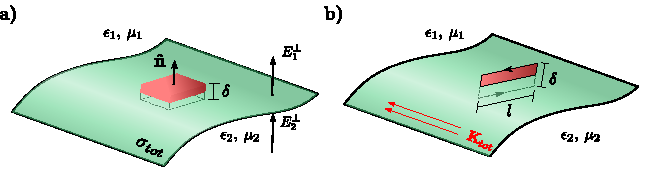
\includegraphics[width=12.5cm]{1-Capitulo-Repaso/0-Diagramas/dibujo.pdf}
	\caption[Condiciones de frontera]{Diagrama de una interfaz (superficie en verde) que separa dos medios distintos. El \textit{medio 1} tiene propiedades ópticas $\epsilon_{1},\,\mu_{1}$, mientras que las del \textit{medio 2} son $\epsilon_{2},\,\mu_{2}$. \textbf{a)} Prisma rectangular con altura $\delta$ y cuyas caras paralelas a la superficie tiene un área $A$. Sobre la superficie que separa a los medios hay una densidad de carga superficial total igual a $\sigma_{tot}$. \textbf{b)} Circuito rectancular con altura $\delta$ y ancho $l$. En la interfaz entre los medios hay una densidad de corriente superficial $\vb{K}_{tot}$.}
	\label{fig:BoundaryConditions} 
\end{figure}
% 
En particular, cuando los medios son lineales, las condiciones de frontera son~\cite{Griffiths}:
\begin{tcolorbox}[title = Condiciones de frontera para materiales lineales]
\begin{equation}
\begin{aligned}
&\epsilon_{1}E_{1}^{\perp}-\epsilon_{2}E_{2}^{\perp}=\sigma_{tot},&\qquad&\vb{E}_{1}^{\parallel}-\vb{E}_{2}^{\parallel}=\vb{0},\\[2pt]
&B_{1}^{\perp}-B_{2}^{\perp}=0,&\qquad& \frac{1}{\mu_{1}}\vb{B}^{\parallel}_{1}-\frac{1}{\mu_{2}}\vb{B}^{\parallel}_{2}=\vb{K}_{tot}\times\vu{n},
\end{aligned}\label{eq:Condiciones_fronteras_lineal}
\end{equation}
\end{tcolorbox}
En las Ecs.~\eqref{eq:Condiciones_fronteras_lineal} es posible notar que, si no hay fuentes externas, tanto componentes paralelas como perpendiculares de los campos EMs son continuas en la frontera entre ambos medios.

\section{Campos eléctromagnéticos armónicos}
Las ecuaciones de Maxwell imponen relaciones entre los cuatro campos $\vb{E}$, $\vb{B}$, $\vb{D}$ y $\vb{H}$. Es posible desacoplar a las ecuaciones de Maxwell y obtener una ecuación para sólo uno de los campos. Para ello, primero, se observa que, en el vacío y sin fuentes externas, es decir, $J_{tot},\:\rho_{tot}=0$, se cumple que
\begin{eqnarray}
	\vb{D}=\epsilon_{0}\vb{E},\qquad\text{y}\qquad\vb{H}=\frac{\vb{B}}{\mu_{0}},
\end{eqnarray}
Por otro lado, se calcula el rotacional de la Ec.~\eqref{eq:maxwell4_mat}
\begin{equation}
	\curl \curl \vb{H}= - \laplacian \vb{H}= \pdv{\curl\vb{D}}{t},\label{eq:1}
\end{equation}
donde se utilizó la relación~\cite{Griffiths}
\begin{equation}
\curl\curl\vb{A}= \grad(\div \vb{A}) - \laplacian \vb{A},\label{eq:propiedad}
\end{equation}
y que $\div \vb{H}=0$. Además, se cumple también que $\curl\vb{D}=-\epsilon_{0}\mu_{0}\pdv{\vb{H}}{t}$. Por tanto, sustituyendo en la Ec.~\eqref{eq:1}, se obtiene que~\cite{Griffiths}
\begin{equation}
\laplacian{\vb{H}}+\epsilon_{0}\mu_{0}\pdv[2]{\vb{H}}{t}=0,\label{eq:ecuacion_de_onda_H}
\end{equation}
A través de un procedimiento análogo se llega a
\begin{equation}
		\laplacian{\vb{E}}+\epsilon_{0}\mu_{0}\pdv[2]{\vb{E}}{t}=0, \label{eq:ecuacion_de_onda_E}
\end{equation}
Las Ecs.~\eqref{eq:ecuacion_de_onda_H} y~\eqref{eq:ecuacion_de_onda_E} son la ecuación de onda vectorial para el campo $\vb{H}$ y $\vb{E}$, respectivamente. Cada una de las componentes de los campos EMs cumplen la ecuación de onda escalar en un medio homogéneo, libre de corrientes y cargas~\cite{BornWolf1980}:
\begin{equation}
	\laplacian V-\frac{1}{c^{2}}\pdv[2]{V}{t}=0,
\end{equation}
en donde $c=1/\sqrt{\epsilon_{0}\mu_{0}}$ corresponde a la velocidad de la luz.

Una de las soluciones más sencillas a la ecuación de onda escalar está dada por~\cite{Griffiths}
\begin{equation}
	V=Ae^{i\left(\vb{k}\cdot\vb{r}-\omega t\right)},\label{eq:funcion_onda}
\end{equation}
donde $\vb{k}$ es el vector de onda, asociado a la dirección de propagación de la onda, y $\omega$ es la frecuencia angular, da el número de vibraciones en $2\pi$ segundos~\cite{BornWolf1980}. La amplitud $A$ es una cantidad compleja. La Ec.~\eqref{eq:funcion_onda} también pudo ser escrita en términos de las funciones seno y coseno, sin embargo, es preferible el uso de exponenciales complejas puesto que es más sencillo de manipular para hacer cálculos. Al final, sólo se considera la parte real de la función de onda~\cite{Griffiths}. A partir de la Ec.~\eqref{eq:funcion_onda} se distingue a la onda plana; se obtiene cuando $\vb{k}\cdot\vb{r}$ es constante, por tanto, en cada instante de tiempo $V$ es constante en cada plano definido por $\vb{k}\cdot\vb{r}$~\cite{Griffiths}. 

Debido a la forma de la dependencia temporal en la Ec.~\eqref{eq:funcion_onda} se dice que el campo es armónico en el tiempo. Por ello, los campos EMs armónicos se escriben como~\cite{Griffiths}
%
\begin{eqnarray}
	\vb{E}_{c}=\vb{E}_{0}e^{i\left(\vb{k}\cdot\vb{r}-\omega t\right)},&&\vb{H}_{c}=\vb{H}_{0}e^{i\left(\vb{k}\cdot\vb{r}-\omega t\right)},\label{eq:Campos_armo}
\end{eqnarray}
con $\omega=kc$. En ausencia de fuentes externas los campos $\vb{E}$ y $\vb{H}$ son ortogonales entre sí y respecto al vector de onda $\vb{k}$, ver Fig.~\ref{fig:EHFields}. Se relacionan entre sí a través de la siguiente ecuación~\cite{Griffiths}:
\begin{equation}
	\vb{H}=\sqrt{\frac{\epsilon_{0}}{\mu_{0}}}\vb{k}\times\vb{E},
\end{equation}

Debido a la forma de los campos EMs [Ecs.~\eqref{eq:Campos_armo}], las ecuaciones de Maxwell se reescriben como~\cite{Bohren}
\begin{equation}
\div \epsilon \vb{E}_{c} = 0, 
\label{eq:maxwell1H}
\end{equation}
\begin{equation}
\div \vb{H}_{c} = 0, 
\label{eq:maxwell2H}
\end{equation}
\begin{equation}
\curl \vb{E_{c}} = i \omega \mu \vb{H}_{c}, 
\label{eq:maxwell3H}
\end{equation}
\begin{equation}
\curl \vb{H}_{c} = -i\omega \epsilon \vb{E}_{c}.
\label{eq:maxwell4H}
\end{equation}
Nuevamente, es posible desacoplar las ecuaciones de Maxwell. Para ello calculamos el rotacional de las Ecs. \eqref{eq:maxwell3H} y \eqref{eq:maxwell4H}:
\begin{equation}
\curl (\curl \vb{E})=i\omega \mu \curl \vb{H} = \omega ^{2} \epsilon \mu \vb{E},
\label{eq:curlE}
\end{equation}
\begin{equation}
\curl (\curl \vb{H})=-i\omega \epsilon \curl \vb{E} = \omega ^{2} \epsilon \mu \vb{H}
\label{eq:curlH}
\end{equation}
Usando la propiedad en la Ec.~\eqref{eq:propiedad}, se reescriben a las Ecs. \eqref{eq:curlE} y \eqref{eq:curlH} como sigue

\begin{tcolorbox}[title = Ecuación vectorial de Helmholtz]\vspace*{-0.3cm}
\begin{subequations}
	\begin{align}
\laplacian \vb{E} + \omega^{2} \epsilon \mu \vb{E}&=0, \label{eq:HelmholtzE}\\
\laplacian \vb{H} + \omega^{2} \epsilon \mu \vb{H}&=0,\label{eq:HelmholtzH}
	\end{align}
\end{subequations}
\end{tcolorbox}
\noindent en donde $k^{2}=\omega^{2} \epsilon \mu$.

\begin{figure}
	\centering
	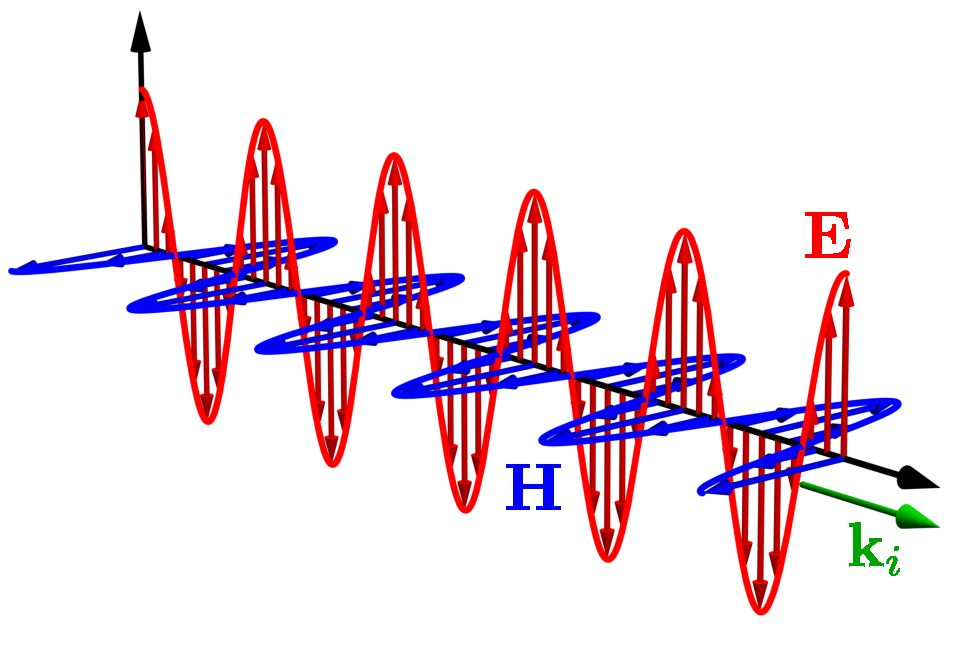
\includegraphics[width=9cm]{1-Capitulo-Repaso/0-Diagramas/campos.pdf}\vspace*{-0.3cm}
	\caption[Campo eléctromagnetico armónico]{Representación de los campos EMs armónico. En rojo se encuentra el campo eléctrico $\vb{E}$ y en azul el campo $\vb{H}$, para cada uno, las flechas indican la orientación de su oscilación. La flecha verde indica la dirección de propagación de la onda, dada por $\vb{k}_{i}$.}\label{fig:EHFields}
\end{figure}
\section{Vector de Poynting}

El vector de Poynting es una cantidad que indica la energía por unidad de tiempo, por unidad de área, transportada por los campos EMs, de forma general, se define como~\cite{Griffiths}:
\begin{equation}
\vb{S}=\left(\vb{E} \cross \vb{H}\right).
\label{eq:poynting}
\end{equation}
La energía por unidad de tiempo que cruza una superficie infinitesimal $\dd{\vb{a}}$ es $\vb{S}\cdot\dd{\vb{a}}$, y es llamado flujo de energía~\cite{Griffiths}.

En el caso de la luz, las longitudes de onda son tan cortas ($\sim 5\times10^{-7}$ m), y el periodo ($\sim10^{-15}$ s), que las mediciones macroscópicas involucran muchos ciclos, por ello no es viable medir directamente al vector de Poynting. Se utiliza el promedio temporal, denotado con $\expval{\quad}$~\cite{Griffiths}. Retomando el caso de campos EMs armónicos, el vector de Poynting luce de la siguiente forma
\begin{equation}
\vb{S} = \Re{\vb{E}_{c}} \cross \Re{\vb{H}_{c}},
\end{equation}
cuyo promedio temporal es~\cite{BornWolf1980}
\begin{equation}
\expval{\vb{S}}=\frac{1}{2}\left(\vb{E}_{c} \cross \vb{H}_{c}^{*}\right),
\label{eq:poynting_promedio}
\end{equation}
en donde $^{*}$ indica el complejo conjugado. El cálculo del promedio temporal se realiza sobre un ciclo completo. Ahora es posible calcular la potencia promedio por unidad de área transportada por una onda EM, es decir, la intensidad~\cite{Griffiths}
\begin{equation}
	I=\expval{S}
\end{equation}

Con el vector de Poynting también se determina la magnitud y dirección de la tasa de transferencia de energía electromagnética en cualquier punto del espacio \cite{Bohren}. Es posible cuantificar la tasa neta con la que la energía EM cruza la frontera de una superficie cerrada $A$ que encierra un volumen $V$~\cite{Bohren}:
\begin{equation}
W=- \int_{A} \vb{S} \vdot \vu{n} \dd A,
\label{eq:rateElecEnergy}
\end{equation}
donde $\vu{n}$ es el vector unitario normal a la superficie. Es importante notar que se agrega un signo menos en la Ec. \eqref{eq:rateElecEnergy} puesto que se ha elegido el vector normal que apunta hacia afuera del volumen. Entonces, si $\vb{S}$ es tal que apunta en la dirección contraria a $\vu{n}$, W será positiva. Lo cual indica que la energía se absorbe. 



